\section{The DiFX correlator}

This document is centered around the NRAO installation of the DiFX \cite{difx} software correlator and its supporting software.
Much of the contents here applies to other installations of DiFX as well, but keep in mind that not a lot of effort is made to generalize these instructions.
Fig.~\ref{fig:block} shows the general data flow-path within the DiFX software correlator system.

\begin{figure}[h]
\begin{center}
\resizebox{5in}{!}{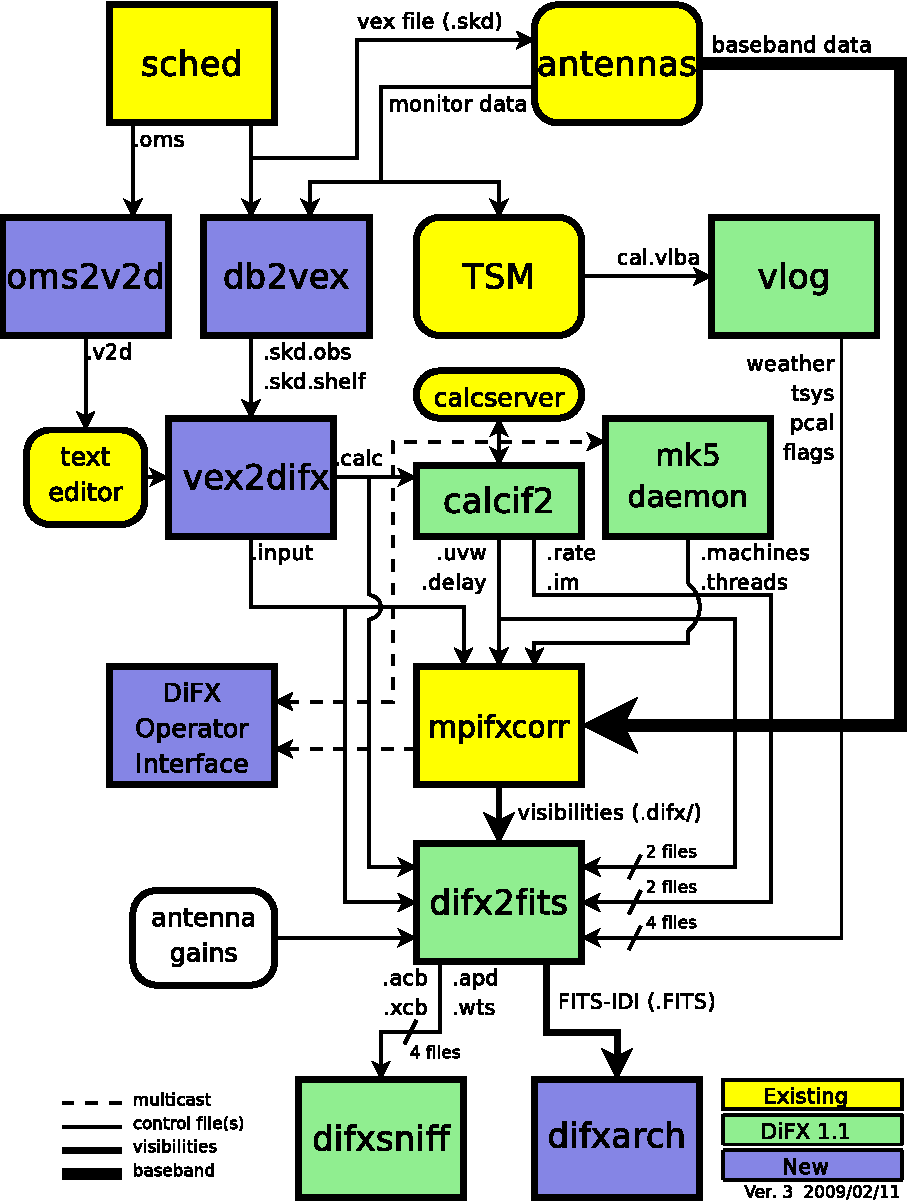
\includegraphics{swcorr_vex_diagram_ver3-crop}}
\caption[blockdiagram]{
{\em The DiFX software correlator block diagram as implemented for the VLBA.}
\label{fig:block}
}
\end{center}
\end{figure}

Past, present, and future versions of DiFX as packaged and used by VLBA operations are described in the following subsections.

% \subsubsection{Supported data formats} \label{sec:formats}


\subsection{NRAO-DiFX 1.0}

Versions 1.0 and 1.1 based correlation on the VLBA hardware correlator job scripts -- the {\tt .fx} files.
This ensures a compatibility period during which both correlators can produce visibilities with expectations of functionally identical results, a feature critical for validation.
This strategy also minimizes the required software effort at its earliest phases.
Version 1.0 came with the following features:
\begin{enumerate}
\item A complete path from {\tt .fx} job scripts to {\tt .FITS} files
\item A command-line only interface
\item Documentation (you are reading it now)
\item Support for VLBA and Mark IV formats
\item Correlation directly off Mark5 modules
\item Support for all projects types except those using special modes, such as pulsars, space VLBI, and near field objects
\item Spectral and time resolution bounded only by practicality
\end{enumerate}
While this version should handle most observations, fast frequency switching and geodesy experiments will produce a large number of output FITS files which may be annoying to observers and the archive.
Version 1.0 was available on February 6, 2008.

\subsection{NRAO-DiFX 1.1}

Version 1.1 builds on version 1.0 and adds the following features:
\begin{enumerate}
\item Used version of {\tt mpifxcorr} that has gone through code merge with the official version
\item Blanking of data replaced by headers (Mark4 format only)
\item Proper data weights
\item Initial Mark5B support
\item Support for oversampled data through decimation
\item Multicast status information for GUI interface
\item Correlation of moving and near field objects
\item Concatenation of multiple output files into a single or multiple FITS-IDI file(s)
\item Better support for jobs with multiple configuration tables
\item Playback off Mark5 modules with missing disks
\item Support for Amazon based Mark5 units
\item Completely replaced the ``Makefile'' system with better integrated alternative
\item Generation of delay model polynomials rather than tables, more like VLBA HW correlator
\item $u, v, w$ values are derived from the delay model (and hence include corrections for aberration, near field observations, and other subtle effects) and are evaluated when writing the FITS file
\item DiFX version accountability
\item Validation of data frames prior to decoding
\item Data evaluation (``sniffing'') built into FITS converter
\end{enumerate}
This version was released on September 3, 2008.
%Features new to version 1.1 are marked with \difxoneone.

\subsubsection{Bugs fixed}

Here are listed some of the more important bug fixes:
\begin{enumerate}
\item The clock offset was used with the wrong sign in the IM table.
\item Printed precision of some important numbers (RA and Dec) was increased.
\item Autocorrelations were ordered incorrectly for observations with a single polarization.
\item The Mark4 format decoder had a 1 day off bug.
\item The Mark4 format decoder had a 64$\times${\it fanout} sample timing offset.
\item Several causes of crashes were fixed; no known crashes remain.
\item Missing VLBA monitor data was handled badly.
\item Due to OpenMPI peculiarity, some processing nodes would get most or all of the work in some cases, which cause the work being done on other nodes to be ignored.  This was fixed by looking for results in a round-robin manner.
\item Integrations that contain data from two adjacent scans are stripped when writing FITS files.
\item Allow FITS files larger than 2GiB in size.
\end{enumerate}

\subsubsection{Known problems}

Known bugs as of the NRAO-DiFX 1.1 release:
\begin{enumerate}
\item The last couple (typically 2) integrations of a job (not a scan) tend to have low weight due to a premature termination of data processing.
\end{enumerate}

\subsection{DiFX 1.5.0}

With DiFX 1.5.0 comes a name change.
Past releases of this series have been known as ``NRAO-DiFX''.
The DiFX community has been largely receptive to the NRAO additions in support of {\tt mpifxcorr} and it was decided that dropping the ``NRAO'' was appropriate.
In some cases the term ``VLBA DiFX'' or ``VLBA DiFX 1.5'' may be mentioned.
These are simply the deployment of DiFX 1.5.0 for the VLBA correlator with some VLBA specific features.
Note that the name given to the VLBA deployment of DiFX is formally ``VLBA DiFX''.

Version 1.5.0 will start allowing correlation of experiments that cannot be represented by {\tt .fx} files and will be based on vex files.
Version 1.5.0 builds on version 1.1 and adds the following features:
\begin{enumerate}
\item Support for using a wide variety of vex files as the basis for correlation.
\item Native ephemeris-based object trajectories are supported.
\item Pulsar gating is supported.
\item Pulsar binning is supported, but not cleanly yet.
\item A graphical user interface is available for correlator operators.
\item The multicast system is fully implemented and is used monitor and control correlation and other operations.
\item Mark5B formatted data, including its 2048 Mbps extension, is supported.
\item The VLBA DiFX Operations Plan \cite{opsplan} is implemented, including interface to the VLBA archive.
\end{enumerate}
Non-NRAO users of DiFX 1.5.0 will still be able to use the tools provided but may not be able to take full advantage of the database back-end without some customization; it is the aim of this document to point out cases where the database is required.
Many of the programs described in previous versions of this document will be upgraded or overtaken by more capable replacements.

Release of DiFX 1.5.0 was announced on June 25, 2009.

Features new to the 1.5 series are marked with \difxonefive.

\subsubsection{Bugs fixed}

Here are listed some of the more important bug fixes:
\begin{enumerate}
\item A rounding issue in {\tt mpifxcorr} occasionally caused the wrong source's UVWs to be assigned.
\item Lower side band data would come out of the sniffer portion of {\tt difx2fits} with the wrong sign for phase, rate, and delay.
\item Different rounding was used to generate start times for {\tt .input} and {\tt .calc} files.
There are no severe consequences of this issue.
\item Scaling in pulsar gating has been made more sane.
\end{enumerate}

\subsection{DiFX 1.5.1}

DiFX 1.5.1 is mostly a bug fix update to version 1.5.0, but with a few new features.
The new features include:
\begin{enumerate}
\item Option to force job breaks (with the break parameter) has been added to {\tt vex2difx}
\item Time/date formats other than decimal MJD are now accepted by {\tt vex2difx}
\item Specification of data files to correlate (rather than Mark5 units) is supported in {\tt vex2difx}
\item Specification of network parameters in {\tt vex2difx} to allow correlation of eVLBI projects
\item {\tt difx2fits} produces a new output file with suffix {\tt .jobmatrix} provides the user with a better idea of the mapping of jobs into {\tt .FITS} files
\item A {\tt vex2difx} mode for generating DiFX files useful for determining pulsar phase has been added
\item EOP values can now be provided within the {\tt .v2d} file
\item Upcoming FITS-IDI keyword WEIGHTYP populated
\item Zero-weight data is not written from {\tt mpifxcorr}
\item New utility {\tt checkdir} to look for oddities in Mark5 module directory files
\end{enumerate}

\subsubsection{Bugs fixed}

Here are listed some of the more important bug fixes:
\begin{enumerate}
\item Concatenation of jobs in the creation of {\tt .FITS} files does the right thing for cases where the antenna subsets change and where antenna reordering is done.
\item The Pulsar Gate Model (GM) {\tt .FITS} file table is now correctly populated for pulsar observations.
\item Autocorrelations are written for each pulsar bin
\item The FXCORR simulator mode of {\tt vex2difx} now selects the correct reference time for antenna clock offsets.
\item A work-around for a Streamstor problem has been added that should improve reliability in Mark5 module correlation when a change in bank is needed.
\item The sign of clock offsets in vex files has been reversed to follow the vex standard
\item Jobs are split at leap seconds
\item LBA data formats are handled more correctly in {\tt vex2difx}
\item The model generator ({\tt calcif2}) now respects polynomial parameters interval and order given on the command line.
\end{enumerate}

DiFX~1.5.1 was made available via subversion on Sep 8, 2009.

\subsection{DiFX 1.5.2}

DiFX~1.5.2 is mostly a bug fix update to version 1.5.1, but with a few new features.
This version of DiFX comes with the following components (and versions): calcif2 (1.1), calcserver (1.2), difx\_db (1.12; NRAO-only), difx2fits (2.6.1), difx2profile (0.1), difxio (2.12.1), difxmessage (0.7), mark5access (1.3.3), mk5daemon (1.2), mpifxcorr (1.5.2), vex2difx (1.0.2), and vis2screen (0.1).
The new features include:
\begin{enumerate}
%\item Primitive support for single-thread VDIF format data
\item Support unmodulated VLBA format data with new pseudo-format ``VLBN''
\item {\tt mpifxcorr} now warns when difxmessage is in use so the user knows why no messages appear on the screen
\item New utility {\tt difxcalculator} in the {\tt difxio} package
\item eVLBI support within {\tt vex2difx}
\item Vastly improved real-time correlation monitoring
\item New utility {\tt diffDiFX.py} to compare two DiFX output files
\item Improved and more consistent error messages (and some of them are now documented!)
\item {\tt vex2difx} now operates in strict parsing mode by default
\item Additional user feedback to indicate suspicious or bad {\tt .polyco} and {\tt .v2d} files
\item {\tt calcif2} warns if any NaNs or Infs are produced
\item Clock adjustments are easier now with {\em deltaClock} and {\em deltaClockRate} parameters in the {\tt vex2difx} antenna settings
\end{enumerate}

\subsubsection{Bugs fixed}

\begin{enumerate}
\item Improve timestamp precision (thanks to John Morgan)
\item The {\tt vlog} program (used at NRAO only, I think) misparsed the pulse cal information in some cases
\item Fixed memory leak in {\tt difx2fits} when combining a large number of jobs
\item Improved FXCORR simulation mode in {\tt vex2difx}
\item Mark5 directory reading systematically generates unique names for all scans even when two scans have the same name
\item Improve reporting of Mark5 errors during playback and change alert severity to be more appropriate
\item Don't overblank certain Mark4 modes (thanks to Sergei Pogrebenko for the bug report)
\item Vex `data valid' period now properly respected
\item Vex clock table tolerance issue corrected
\item Changes in Mark5 mode should be safer (note that currently {\tt vex2difx} never exercises multiple modes in a single job)
\item When making the cross spectrum sniffer plots, respect the reference antenna
\item Improved pulsar polynomial file error checking is performed
\item Amplitude-phase-delay (APD) sniffer plots always have refant first when multiple refants are supplied
\item Project name should now appear on sniffer APD plots
\item Mark5 units now send status information even when no playback is occuring (eliminating the incorrect {\tt LOST} state issue as displayed in the DOI)
\end{enumerate}

\subsubsection{Known problems}

\begin{enumerate}
\item Extensive use in VLBA operations has shown that occasional data dropouts of one or more antenna, sometimes in a quasi-repeatable manner, affect completeness of some jobs.  
It is not clear exactly what the cause is at this point, however its cure is a high priority.
\item Loss of a few FFTs of data will occur in rare circumstances.
\item Clock accountability is poor when jobs containing multiple clock models for antennas are combined.
\end{enumerate}

DiFX~1.5.2 was made available via subversion on Jan 20, 2010.

\subsection{DiFX~1.5.3}

DiFX~1.5.3 is mainly intended as a bug fix update to version~1.5.2, though some new features have made their way into the codebase.
This version of DiFX comes with the following components (and versions): calcif2 (1.3), calcserver (1.3), difx\_db (1.13; NRAO-only), difx2fits (2.6.2), difx2profile (0.2), difxio (2.12.2), difxmessage (7.2), mark5access (1.3.4), mk5daemon (1.3), mpifxcorr (1.5.3), vex2difx (1.0.3), and vis2screen (0.2).
Many changes are motivated by issues found running DiFX full time in Socorro.

The new features include:
\begin{enumerate}
\item Mark5 directory ({\tt .dir}) files can contain {\tt RT} on the top line to indicate the need to play back using {\em Real-Time} mode.
\item {\tt difxqueue} (NRAO only) now takes an optional parameter specifying the staging area to use.
\item New Mark5 diagnostic programs ({\tt vsn} and {\tt testmod}) introduced to wean off the use of the {\tt Mark5A} program.
\item {\tt mk5daemon} can now mount and dismount USB and eSATA disks through mk5commands.
\item {\tt mk5cp} now makes the destination directory if it doesn't exist.
\item {\tt mk5daemon} will now warn if free disk space is getting low.
\item {\tt db2vex} (NRAO only) now allows field station logs to be provided.  As of now, only media VSNs are extracted.
\item Playback off Mark5 units has been made more robust with better error reporting.
\item New utility {\tt m5fold} that can be used to look at repeating signals in baseband data total power (e.g., switched power)
\item {\tt vex2difx} now supports job generation in cases where upper side band was observed at one antenna and lower sideband at another.
\end{enumerate}

\subsubsection{Bugs fixed}

\begin{enumerate}
\item Don't unnecessarily drop any FFTs of data.
\item Sub-integrations longer than one second could cause integer overflows.
\item Fix bug in {\tt vex2difx} where jobs were not split at clock breaks.
\item {\tt difx2fits} was guilty of incorrect clock accoutability after a clock change at a station when merging multiple jobs.  Worked around by not allowing such jobs to merge.
\item {\tt db2vex} (NRAO only) warns when more than one clock value is found for an antenna.
\item Mark5 unit bank switches now routinely call {\tt XLRGetDirectory()} to work around a newly discovered bug in the StreamStor software.
\item A couple possible memory leaks in the mark5access library were fixed (thanks Alexander Neidhardt and Martin Ettl).
\item Lots of compiler warnings quashed (mostly of the ``unused return value'' kind).
\item Olaf Wuchnitz found two FITS file writing problems in {\tt difx2fits} dating back to code inherited from FXCORR!
\item Two more digits are retained for the time and one more digit is retained for amplitude information in the {\tt .apd} and {\tt .apc} sniffer files.
\item Some bugs related to replacement of special characters by ``entities'' in XML messages are fixed.
\item New traps are in place in many places to catch string overruns.
\item Fix for writing {\tt .calc} files with more than one ephemeris driven object.
\item {\tt vex2difx} would get {\em very} slow due to constantly sorting a list of events.  Now this list is only sorted when necessary, drastically speeding it up.
\item The {\tt RCfreqId} parameter in the difxdatastream structure (in difxio) was used with two different meanings that are normally the same.  Cases where they differred caused exceptions.  Fixed in difxio and difx2fits. (Thanks to Randall Wayth for leading to the discovery)
\item {\tt difx2fits} would assign a bogus {\tt .jobmatrix} filename when not running the sniffer.
\item {\tt vex2difx} could get caught in an infinite loop when making jobs where two disk modules had zero time gap.
\item {\tt difx2fits} used a bad config index when making the puslar GM table when multiple configs were present.
\item Within {\tt mpifxcorr} an extra second was added to the validity period for polycos to ensure no gap in coverage.
\item {\tt mk5dir} would add correct the date improperly for Mark4 formats after beginning of 2010.
\item Lots of fixes for building FITS files out of a subset of baseband recorded channels.
\item FITS files now support antennas with differing numbers of quantization bits.
\item Lots of Mac OS/X build issues fixed.
\end{enumerate}

DiFX 1.5.3 was released on April 16, 2010.

\subsection{DiFX~1.5.4}

DiFX~1.5.4 is likely the last 1.5 series formal release of DiFX, though an additional release could be made if demand is there.

The new features include:
\begin{enumerate}
\item {\tt difx2fits} can now produce FITS files with only a subset of the correlated sub-bands.
\item {\tt difx2fits} can be instructed to sniff on an arbitrary timescale.
\item The {\tt makefits} wrapper for {\tt difx2fits} now respects a -B option for phase bin selection.
\item {\tt difxio} has improved checking that prevents merging of jobs with incompatible clocks.
\item {\tt difxio} now maintains a separate clockEpoch parameter for each antenna.
\item {\tt difxStartMessage} now contains DiFX version to run, allowing queued jobs to be run under different DiFX versions.
\item The curses utilities {\tt mk5mon} and {\tt cpumon} now catch exceptions and can be resized without infecting the terminals they are run in.
\item New sub-library called mark5ipc added that provides a semaphore lock for Mark5 units.
\item The {\tt testdifxmessagereceive} utility can now filter on message types.
\item Support for SDK9 throughout (e.g., in {tt mpifxcorr}, {\tt mk5daemon}, and other utilites).
\item Support for new Mark5 module directory formats (Haystack Mark5 memo 81).
\item Several new Mark5 utilities to make up for Mark5A functionality that will not longer be available: {\tt vsn}, {\tt testmod}, {\tt recover}, {\tt m5erase}.
\item {\tt mk5cp} can now copy data based on byte range.
\item Many programs directly talking to the StreamStor card of Mark5 units use WATCHDOG macros for improved diagnostics when problems occur.
\item More protection against incomplete polyco files added to {\tt mpifxcorr} (Note: should add this to {\tt vex2difx} as well).
\item The GUI can now spawn different DiFX versions at will through the use of difxVersion parameter in the DifxStartMessage and wrapper scripts.
\item {\tt difx2fits} can now convert LSB to USB for matching purposed.  When used, all LSB sub-bands must have corresponding USB sub-bands on one or more other antenna.
\item {\tt mark5access}-based utilities (e.g., {\tt mp5spec}) can now read from stdin.
\item New utility {\tt mk5cat} can send data on a Mark5 module to stdout.
\end{enumerate}

\subsubsection{Bugs fixed}

\begin{enumerate}
\item Only alt-az telescopes received the correct model.  Fixed.  Note that CALC and FITS-IDI don't have a good match between their sets of allowed mount types.
\item {\tt difx2fits} now properly propagates quantization bits on a per antenna basis.
\item Logic errors in {\tt difxio} would confuse {\tt difx2fits} in cases where different antennas use different frequency setups.  Fixed.
\item Weights are blanked in {\tt difx2fits} prior to populating each record, preventing screwy weights for unused sub-bands.
\item {\tt vex2difx} would sometimes hang or not converge on job generation.  Fixed.
\item {\tt vex2difx} now doesn't assume source name is same as vex source def identifier.
\item {\tt mpifxcorr} generated corrupted weights and amplitudes when post-FFT fringe rotation was done.  Fixed.
\end{enumerate}

\subsection{Known bugs}

\begin{enumerate}
\item Tweak Integration Time feature of {\tt vex2difx} often does the wrong thing.
\end{enumerate}

DiFX 1.5.4 was released on October 12, 2010.

\subsection{DiFX 2.0.0}

DiFX 2.0.0 is based on an upgraded {\tt mpifxcorr} that breaks {\tt .input} file compatibility with the 1.0 series.
This new version will allow more flexible correlation of mis-matched bands and correlation at multiple phase centers along with general performance improvements.
Development of the 2.0 capabilities will occur in parallel with the 1.0 series features.

\subsubsection{New features}

\begin{enumerate}
\item Pulse cal extraction in {\tt mpifxcorr}.
\item Massive multi-phase center capabilitiy.
\item New utitility {\tt zerocorr} added.
\item External pulse cal extraction utility {\tt m5pcal} added.
\item DiFX output format is all-binary, meaning speed and disk savings
\end{enumerate}

\subsection{Known bugs}

\begin{enumerate}
\item Zoom band support has multiple problems.
\end{enumerate}

DiFX 2.0.0 was released on October 12, 2010.

\subsection{DiFX 2.0.1}

DiFX 2.0.1 is a bug fix and clean-up version in response to numerous improvements to DiFX 2.0.0.
There are a number of new features as well.

\subsubsection{New features}

\begin{enumerate}
\item New utility {\tt checkmpifxcorr} to validate DiFX input files
\item Switched power detection in {\tt mpifxcorr}
\item Early multi-thread VDIF format support
\item RedHat RPM file generation for some packages (can extend to others on request)
\item Improvements to method of selecting which pulse cal tones get propagated to FITS
\item Initial complex sampling support
\item Improved locking mechanism for direct mark5 access (using IPC semaphores; difxmessage)
\end{enumerate}

\subsubsection{Bug fixes}

\begin{enumerate}
\item Fix model accountability bug in difx2fits when combining jobs
\item Numerous fixes for zoom bands (in {\tt mpifxcorr}, {\tt vex2difx} \& {\tt difx2fits})
\item Native Mark5 has improved stability for cranky modules
\item Numerous fixes for DiFX-based phase cal extraction (mostly in {\tt difx2fits}, mostly for multi-job)
\item Fractional bit correction for a portion of lower sideband data got broken in difx 2.0.0. Fixed.
\item Migrate {\tt difxcalculator} to DiFX 2; was not complete for DiFX 2.0.0
\end{enumerate}

DiFX 2.0.1 is expected to be released in April 2011.

\subsection{Features left to implement}

Here is a list of other features to add to DiFX that are not directly tied to any particular version:
\begin{enumerate}
\item Full VDIF support
\item Support for K5 format
\item Pulsar bins with proper output format
\item Fast-forwarding over unneeded data in the native Mark5 module datastream
\item Phase cal extraction
\item Space VLBI support
\item Switched power extraction
\item Playback of two independent modules in one Mark5 unit
\item Non-bank-mode Mark5 support
\item Spectral selection between FFT and cross-correlation to allow for greater spectral resolution
\item Conversion of DiFX output to Mark4 correlator format
\item Support for antenna local oscillator offsets
\end{enumerate}

\subsection{DiFX and AIPS}

Only one task in AIPS, {\tt FITLD}, has to deal with the telescope/correlator specific aspect of the FITS-IDI files that the VLBA correlator and DiFX generate.
The FITS-IDI variant of FITS was first documented in AIPS Memo 102 \cite{aips102}, and more recently in AIPS Memo 114 \cite{aips114}, which will be generally available shortly.
It has been modified for better support support of DiFX FITS output.
In general, these changes make {\tt FITLD} less telescope specific so the resulting FITS-IDI files from any DiFX installation should be highly compatible with AIPS.
Several changes have been made to the 31DEC08 AIPS as a result of DiFX testing:
\begin{enumerate}
\item Correction for digital {\it saturation} in auto-correlations is disabled for DiFX FITS files.  See \cite{sci12} for some details on this correction which is not needed for DiFX data.
\item Support for FITS-IDI files greater than 2~GiB in size.
\item Weather table was not populated properly.
\item FITS files with multiple UV tables would generate incomplete GEODELAY columns in CL tables (not relevant to DiFX).
\end{enumerate}
It is recommended that your AIPS installation be kept up to date.

With the following exceptions, data reduction of DiFX correlated data should be identical to that of VLBA hardware correlator data.
This includes the continued use of {\tt DIGICOR=1} in {\tt FITLD} and the use of {\tt ACCOR} as you would have for the hardware correlator.
The exceptions are:
\begin{enumerate}
\item Use of {\tt FXPOL} to correct data ordering in the case of {\em half} polar (e.g., {\tt RR} and {\tt LL} products) is no longer needed.
\item Use of {\tt VBGLU} to concatenate data sets in the case of 512~Mbps observations is no longer needed.
\item Data is usually combined into a single FITS-IDI file with proper calibration data attached, usually implying that {\tt TBMRG} is not needed to properly concattenate calibration data.  This makes DiFX FITS-IDI data similar to the {\em pipeline-processed} VLBA data that was made available to users of the hardware correlator with the difference being that the original FITS-IDI format is retained, keeping file sizes typically 25\% smaller. 
\end{enumerate}
These changes should make data processing easier in almost all circumstances.
